 
\documentclass{beamer}
\setbeamertemplate{section in toc}[sections numbered]
\usefonttheme[onlymath]{serif}
\beamertemplatenavigationsymbolsempty
\setbeamertemplate{footline}{% 
  \hfill% 
  \usebeamercolor[gray!50]{page number in head/foot}% 
  \usebeamerfont{page number in head/foot}% 
  \insertframenumber\,/\,\inserttotalframenumber%
}
\usepackage{amsmath}
\usepackage{graphicx}
% \usepackage{caption}
% \usepackage[skip=0pt]{subcaption}
% \usepackage[tight,FIGTOPCAP]{subfigure}
\usepackage{lmodern}
\usepackage[round]{natbib}
\usepackage{braket}
\usepackage{color}
\usepackage{bm}
\usepackage{amssymb}
\usepackage{bbold}
\usepackage{tikz}
\usepackage{empheq}
\usepackage{stackengine}
\usepackage{framed}
\usepackage[percent]{overpic}
\usepackage{adjustbox}
\DeclareMathOperator{\sgn}{sgn}
\tikzset{>=latex}
\newcommand{\blue}[1]{{\color{blue}{#1}}}
\newcommand{\md}{\mathrm{d}}
\newcommand{\ms}{\mathsf}
\newcommand{\bs}{\boldsymbol}
\newcommand{\mc}{\mathcal}
\renewcommand{\(}{\left(}
\renewcommand{\)}{\right)}
\renewcommand{\[}{\left[}
\renewcommand{\]}{\right]}

%Information to be included in the title page:
\title{Toric Code}
%\author{Apoorv Tiwar, Ammar Jahin, and Yuxuan Wang}
%\institute{University of Florida}
\date{University of Florida, \today}

\begin{document}
\frame{\titlepage} 
\AtBeginSection[]
{
\begin{frame}
    \frametitle{Outline}
    \tableofcontents[currentsection]
\end{frame}
}



\begin{frame}
    \frametitle{Recap of last time}

    \begin{itemize}
        \item Error detection big picture: \begin{enumerate}
            \item Add redundancy $k \rightarrow n$ qubits: $\ket{\psi} \rightarrow \ket{\psi}_L$
            \item Errors: $\ket{\psi}_L \rightarrow E_L\ket{\psi}_L$ 
            \item Considering only X-type and Z-type errors is enough to account for all errors.
            \item Add ancilla and measure the ancilla 
        \end{enumerate}
        \item Stabilizer codes: \begin{enumerate}
            \item $\mc C = \text{span}\{\ket{\psi}_L \in \mc H : \ S_i\ket{\psi}_L = \ket{\psi}_L \}$
            \item $S_i^2 = 1$
            \item For error detection, $\{E_L,S_i\} = 0$ for at least one $S_i$. 
            \item Syndrome extraction: $(1+S_i)E_L \ket{\psi}_L \ket{0} + (1-S_i)E_L \ket{\psi}_L \ket{1}$
        \end{enumerate} 
        
    \end{itemize}

\end{frame}

\begin{frame}
    \frametitle{Two approaches to Kitaev toric code \citep{Kitaev_2003}}

    \begin{columns}
        \begin{column}{0.5\textwidth}
            \begin{center}
            As a discrete gauge theory
            \end{center}
        \end{column}
        \begin{column}{0.5\textwidth}
            \begin{center}
            As a quantum code
            \end{center}
        \end{column}
    \end{columns}

    \begin{columns}
        \begin{column}{0.5\textwidth}
            \begin{itemize}
                \item It's a $\mathbb{Z}_2$ gauge theory
                \item It has anyonic excitations
                \item Long range entanglement and topological order
            \end{itemize}
        \end{column}
        \begin{column}{0.5\textwidth}
            \begin{itemize}
                \item It implements a specific type of quantum code
                \item Allow error detection and error correction
                \item Allows for a restricted qubit operations
            \end{itemize}
        \end{column}
    \end{columns}
    \vspace{10pt}
    
    \begin{center}
        \begin{framed}
            This talk will focus on the quantum code aspect. 
            \end{framed}
    \end{center}
\end{frame}

\begin{frame}
    \frametitle{Outline}

    \tableofcontents

\end{frame}

\section{Kitaev toric code}
\subsection{The model}
\begin{frame}
    \frametitle{Kitaev Toric Model}
    \begin{columns}
        \begin{column}{0.67\textwidth}
            \begin{itemize}
                \item A lattice model of spin-$1/2$ particles.
                \item Each unit cell has $2$ spin sites, $1$ and $2$.
                \item Local operators: $\{\vec{\sigma}_{1}(\bm R_i), \vec{\sigma}_{2}(\bm R_i)\}$
                \item Operators at different lattice sites commute.
            \end{itemize} 
        \end{column}
        \begin{column}{0.33\textwidth}
            \centering
            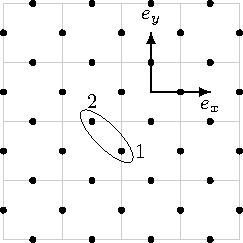
\includegraphics[scale=0.8]{spin_grid.pdf}
        \end{column}
    \end{columns}
    \pause
    \vspace{8pt}
    \begin{columns}
        \begin{column}{0.62\textwidth}
            The Hamiltonian: 
                \begin{align*}
                    H =& -\sum_{\bm R_i} \(A(\bm R_i)  + B(\bm R_i) \)\\
                    A(\bm R_i) = \ &\sigma^x_{2}(\bm R_i)\sigma^x_{1}(\bm R_i) \\  & \sigma^x_{2}  (\bm R_i + e_x)\sigma^x_{1} (\bm R_i+ e_y), \\
                    B(\bm R_i) = \ & \sigma^z_{1} (\bm R_i)\sigma^z_{2} (\bm R_i) \\ &\sigma^z_{1} (\bm R_i - e_x)\sigma^z_{2} (\bm R_i - e_y) 
                \end{align*}
        \end{column}
        \begin{column}{0.38\textwidth}
            \centering
            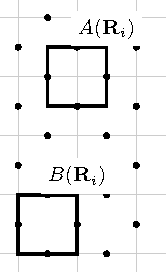
\includegraphics[scale = 1, trim=0 0 0 0, clip]{elementry_loops.pdf}

        \end{column}
    \end{columns}
\end{frame}

\begin{frame}
    \frametitle{Ground state of the Kitaev model}
    \begin{center}
        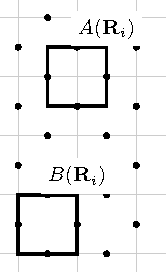
\includegraphics[scale = 1, trim=0 65 0 0,clip]{elementry_loops.pdf} \quad \quad 
        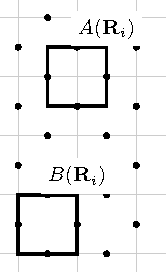
\includegraphics[scale = 1, trim=0 8 0 65,clip]{elementry_loops.pdf}
    \end{center}
    Notation: 
    
    $\sigma^x$: line perpendicular to unit cell edge at the spin site.

    $\sigma^z$: line along the unit cell edge at the spin site.
    \pause
    \begin{itemize}
        \item $A(\bm R_i)$ and $B(\bm R_i)$ are two different \emph{loops} in the system. 
        \item They only look like loops because of our choice of notation.
        \item No need for arrows on the loops.
        \item $A^2(\bm R_i) = 1$ and $B^2(\bm R_i) = 1$. Both have eigenvalues of $\pm 1$.
        \item $\[A(\bm R_i), B(\bm R_i)\] = 0$
    \end{itemize}
    \pause
    Ground sates $\ket{\Omega_0}$ of $H = -\sum_{\bm R_i} \(A(\bm R_i)  + B(\bm R_i) \)$ is defined by, 
    \begin{align*}
        A(\bm R_i)\ket{\Omega_0} = \ket{\Omega_0}, \  B(\bm R_i)\ket{\Omega_0} = \ket{\Omega_0}
    \end{align*}
\end{frame}


\subsection{The code}
\begin{frame}
    \frametitle{The code}
    We consider a $N \times N$ lattice on a torus. 
    \begin{itemize}
        \item The Hilbert space, $\mc H$, is $2^{2N^2}$ dimensional. 
        \item Codeword space, $\mc C$, is defined as \begin{align*}
            \mc C = \text{span}\{\ket{\Omega_0} \in \mc H : A(\bm R_i)\ket{\Omega_0} = \ket{\Omega_0}, \ B(\bm R_i)\ket{\Omega_0} = \ket{\Omega_0} \}
        \end{align*}
        \item This quantum code is called TOR($N$), the toric code.
        \item $A(\bm R_i)$, and $B(\bm R_i)$ are the code stabilizers. 
    \end{itemize}
    \pause
    \begin{columns}
        \begin{column}{0.8\textwidth}
            \begin{itemize}
                \item There are $2N^2 - 2$ independent stabilizers. There are $N^2$ $A(\bm R_i)$, and $N^2$ $B(\bm R_i)$ operators, but we have the following dependencies, \begin{align*}
                    \prod_{\bm R_i} A(\bm R_i) = 1, \prod_{\bm R_i} B(\bm R_i) = 1 \leftarrow  \text{No edges left.}
                \end{align*} 
                \item $\mc C$ is $(2^{2N^2})/(2^{2N^2-2}) = 2^2$ dimensional. It can encode 2 qubits. 
            \end{itemize}
        \end{column}
        \begin{column}{0.2\textwidth}
            \vspace{25pt}
            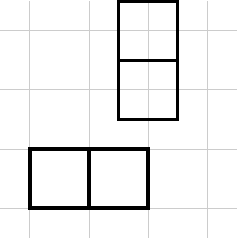
\includegraphics[scale = 0.6, trim=7 0 7 0,clip]{in_two_a_b.pdf}  
        \end{column}
    \end{columns}
\end{frame}
\begin{frame}
    \frametitle{What labels the ground states}
    Since the code stabilizers defines $2^{2N^2-2}$ 4D subspaces, we must label the $4$ states within each subspace by  other independent operators that commute with all the $A(\bm R_i)$ and $B(\bm R_i)$. 
    \pause
    \begin{columns}
        \begin{column}{0.55\textwidth}
            \begin{itemize}
                \item Every contractible loop can be decomposed into smaller loops of $A(\bm R_i)$ or $B(\bm R_i)$. 
                \item There are 4 different non-contractible loops. 
                \item $\{Z_1, Z_2, X_1, X_2\}$ commute with all contractible loops. 
                \item $\{Z_1, X_1\} = 0 $, $\{Z_2, X_2\} = 0 $
                \item The entire $2^{2N^2}$ Hilbert space can be labeled by the eigenvalues of, $\{Z_1, Z_2, A(\bm R_i), B(\bm R_i)\}$
            \end{itemize}
        \end{column}
        \begin{column}{0.45\textwidth}
            \vspace{10pt}
            \centering
            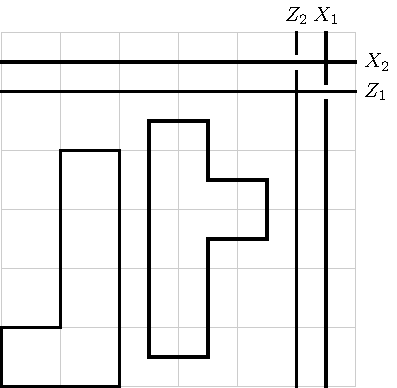
\includegraphics[scale=0.7, trim=0 0 0 0,clip]{decomp_loops.pdf}
        \end{column}
    \end{columns}
    
\end{frame}

\begin{frame}
    \frametitle{Errors}
    A general error can be any linear combination of,
    \begin{align*}
        E(\{\alpha^{l}_i, \beta^{m}_j\}) = \prod_{\substack{\bm R_i, \bm R_i\\ l, m}} (\sigma^x_l(\bm R_i))^{\alpha^{l}_i} (\sigma^z_m(\bm R_j))^{\beta^m_j},
    \end{align*}
    \pause
    % There are a total of $2^{2N^2+1}$. 
    These can be divided broadly into 3 categories: 
    \begin{enumerate}
        \item Contain only closed contractible loops. $E_1$.
        \item Contain one or more open strings. $E_2$.
        \item Contain one or more closed non-contractible loops. $E_3$.
    \end{enumerate}
    \pause
    \begin{itemize}
        \item Errors of type 1 are not errors at all, $E_1\ket{\Omega_0} = \ket{\Omega_0}$.
        \item Errors of type 2 can be detected by a syndrome measurement. 
        \item Errors of type 3 cannot be detected. 
    \end{itemize}
    \pause
    \begin{framed}
        Errors of type 3, must at least be $N$ long. And assuming errors act independently on each qubit, these errors would be exponentially suppressed, $e^{-\alpha N}$
    \end{framed}
\end{frame}
\begin{frame}
    \frametitle{Error detection, and correction}

    Open string operations anticommute with two stabilizer operators, one surrounding each end of the open ended loop.  
    \begin{columns}
        \begin{column}{0.5\textwidth}
            \begin{align*}
                B(\bm R_i) E_2 \ket{\Omega_0} = -E_2 \ket{\Omega_0}, \\ 
                \\
                A(\bm R_j) E_2 \ket{\Omega_0} = -E_2 \ket{\Omega_0}.
            \end{align*}
        \end{column}
        \begin{column}{0.5\textwidth}
            \centering
            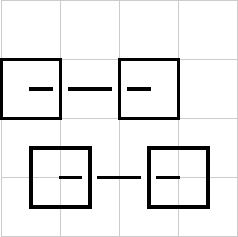
\includegraphics[scale=0.9]{open_closed_loop.pdf}
        \end{column}
    \end{columns}
    \pause
    \begin{itemize}
    \item These errors can be detected using a syndrome measurements. 
    \item Notice that $E_2\ket{\Omega_0}$ are excited states of the Hamiltonian, with $\Delta E \geqslant 2$. 
    \item Kitaev also suggested fixing these errors by coupling the system to a heat bath and cooling the system down. 
    \end{itemize}
    
\end{frame}

% \begin{frame}
%     \frametitle{Local perturbations}

%     It's important to check if the system is stable under local perturbations, otherwise the ground states might split and the system would lose the information encoded into its ground states.  
%     \begin{align*}
%         V =  - \sum_{\substack{\bm R_i, l}} \vec{h} \cdot \vec{\sigma}_{l}(\bm R_i) - \sum_{\substack{\bm R_i, \bm R_j \\ l, m }} \vec{\sigma}^{T}_{m}(\bm R_j) J^{m l}(\bm R_j, \bm R_i)\vec{\sigma}_{l} (\bm R_i)
%     \end{align*}

%     Splitting caused by this perturbation is $e^{-aN}$, for some finite $a$. 
% \end{frame}

\subsection{How to perform logical operations}

\begin{frame}
    \frametitle{Excitations of the toric code}
    Let's look at low energy excitations of the toric code. 
    \begin{itemize}
        \item We cannot have excitation with $\Delta E = 1$. This would violate 
        \begin{align*}
            \prod_{\bm R_i} A(\bm R_i) = 1, \ \ \prod_{\bm R_i} B(\bm R_i) = 1.
            \end{align*}\
        \item The lowest energy excitations have $\Delta E = 2$ and are obtained by applying string operators to the ground states. 
    \end{itemize}
    \pause
    \begin{center}
        \begin{columns}
            \begin{column}{0.5\textwidth}
                $S^x(t)\ket{\Omega_0},\  S^z(t)\ket{\Omega_0}$,
                which depend on
                \begin{enumerate}
                    \item The two end points
                    \item The homotopy of string connecting the two ends, how many non-contractible loops it make. Not the detailed path. 
                \end{enumerate}
            \end{column}
            \begin{column}{0.5\textwidth}
                \centering
                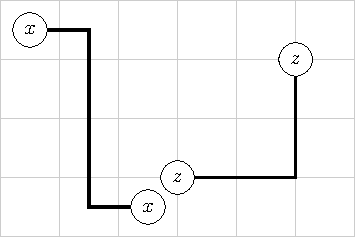
\includegraphics[scale = 0.8]{two_strings.pdf}
            \end{column}
        \end{columns}
    \end{center}
\end{frame}

\begin{frame}
    \frametitle{Allowed logic operaion using kitaev model}
    The non-contractible loops of the toric code behave as Pauli matrices acting on two qubits:
    \begin{align*}
        \[Z_1, Z_2 \] = 0  \ \ \ \ \[X_1, X_2 \] = 0 \ \ \ \ \{Z_1, X_1 \} = 0  \ \ \ \ \{Z_2, X_2 \} = 0 
    \end{align*}
    \begin{enumerate}
        \item $Z$ operation. 
        \begin{itemize}
            \item Create an a $z$-type particles pair. 
            \item Move one around one non-contractible loop. The direction determine which qubit get acted on. 
            \item Annihilate the two particles. 
        \end{itemize}
        \item $X$ operation. Using the same steps but with an $x$-type particle. 
    \end{enumerate}
    These operations do not give us a universal quantum computer. 
\end{frame}

\begin{frame}
    \frametitle{The dual lattice}

    For the same arrangement of spins there are two ways of defining the lattice. Both of them are equally valid. 
    \begin{columns}
        \begin{column}{0.55\textwidth}
            \begin{itemize}
                \item This highlights an important property of the system. 
            \end{itemize}
            Let $R_y(\theta)$ be the rotation operation around the $y$-axis then: 
            \begin{align*}
                R_y(90^\circ) A(\bm R_i) R^{-1}_y(90^\circ) = B^\prime(\bm R_i) \\
                R_y(90^\circ) B(\bm R_i) R^{-1}_y(90^\circ) = A^\prime(\bm R_i)
            \end{align*}
        \end{column}
        \begin{column}{0.45\textwidth}
            \begin{center}
            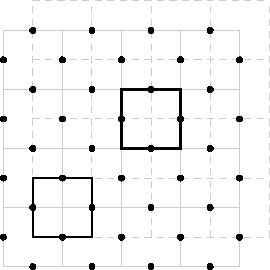
\includegraphics[scale=0.9]{dual_lattice.pdf}
            \end{center}
        \end{column}
    \end{columns}

    \begin{framed}
    This operation takes an $x$-type particle to a $z$-type particle. 
    \end{framed}

\end{frame}
\section{Anyonic nature of the excitations}
\begin{frame}
    \frametitle{The toric code in different geomtries}
    A (surprising) aspect about the toric code is that the ground state degeneracy depends on the genus, $g$, of the manifold. The toric code is $4^g$ degenerate. 
    
    \pause
    On a \emph{sphere} there are no non-contractible loops. $A(\bm R_i)$ and $B(\bm R_i)$ can label the entire Hilbert space. 
    \begin{columns}
        \begin{column}{0.5\textwidth}
            \begin{itemize}
                \item Hilbert space is $2^{12N^2}$ dimensional.
                \item $6N^2 \ B(\bm R_i)$ operators.
                \item $6N^2 + 2 \ A(\bm R_i)$ operators.
            \end{itemize}
        \end{column}
        \begin{column}{0.5\textwidth}
            \centering
            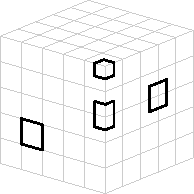
\includegraphics[scale=1.1]{toric_on_sphere.pdf}
        \end{column}
    \end{columns}
    \pause
    \begin{framed}
        The dependance of the ground state degeneracy on the geometry of the manifold is one of the defining features of topological order. 
    \end{framed}
\end{frame}
\begin{frame}
    \frametitle{Particle content of the toric code}
    \begin{columns}
        \begin{column}{0.85\textwidth}
            \begin{itemize}
                \item No particles, 1.
                \item $z$-type particle, referred to as electric charge, $e$.
                \item $x$-type particle, referred to as a magnetic vortex, $m$.
                \item A combinations of an $e$ and an $m$ particle, $\psi = e \times m$
                \item For convince we drop the lattice from the background, and distinguish different strings by different colors.
            \end{itemize}
        \end{column}
    \begin{column}{0.15\textwidth}
        \centering
        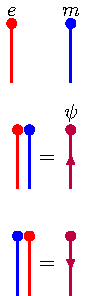
\includegraphics[scale=1]{kinds_of_particles.pdf}
    \end{column}
    \end{columns}
    \pause
    \vspace{10pt}
    Next we ask what is the statistics of these particles. 

    \begin{itemize}
        \item It's natural to consider a braid group because of the strings attached to the particles.
        \item There are three kinds of strings. The group is then said to be a colored braid group. 
    \end{itemize}    
\end{frame}

\begin{frame}
    \frametitle{Rules and fusion rules}
    \begin{columns}
        \begin{column}{0.6\textwidth}
            \begin{itemize}
                \item The electric charge, $e$ is a boson. 
                \item The magnetic vortex, $m$ is a boson. 
                \item $e$ going around $m$ gives a $-1$. 
                \item $\psi$ is a fermion.
                \item The braid group is Abelian. 
            \end{itemize}
        \end{column}
        \begin{column}{0.4\textwidth}
            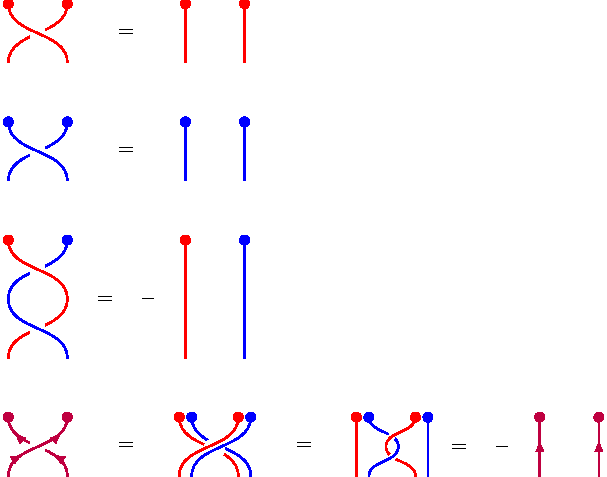
\includegraphics[scale=0.9, trim=0 60 170 0, clip]{rules_of_braiding.pdf}
        \end{column}
    \end{columns}
    \vspace{10pt}
    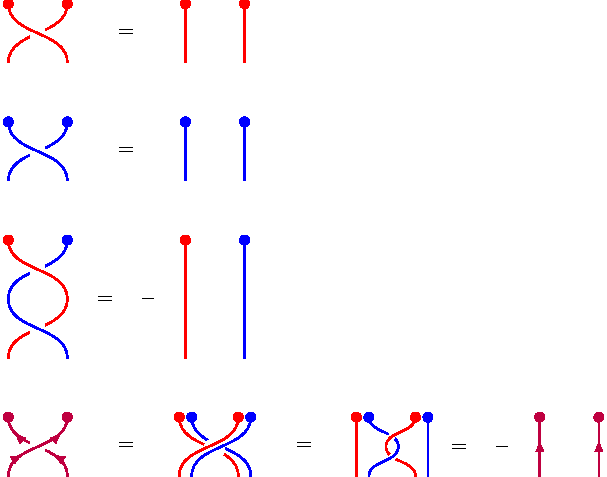
\includegraphics[scale=1, trim=0 0 0 190, clip]{rules_of_braiding.pdf}
\end{frame}

\begin{frame}
    \frametitle{Anyons front and center}
    \framesubtitle{Anyons implies the ground state degeneracy.}

    \begin{framed}
        We can think of the how the anyons braid, as defining the topological order in the system.
    \end{framed}
    \begin{itemize}
        % \item Let $Z_{i}\ (X_{i})$ be the operation that create an $m\ (e)$ particle pair, take one of them around one of the non-contractible loops of the torus, and annihilate the pair again. 
        \item The ground state(s) is a sate with no particles in it. If $\ket{\Omega_0}$ is a ground state, so are $Z_i \ket{\Omega_0}$ and $X_i \ket{\Omega_0}$.
    \end{itemize}
    \begin{itemize}
        \item Braiding rules implies \begin{enumerate}
            \item $Z^2_1 + Z^2_2 + X^2_1 + X^2_2 = 1$
            \item $\[Z_1, Z_2 \] = \[X_1, X_2 \] = 0$
            \item $\{Z_1, X_1 \} = \{Z_2, X_2 \} = 0$.
        \end{enumerate}
        \item This implies the ground state is fourfold degenerate. 
    \end{itemize}
    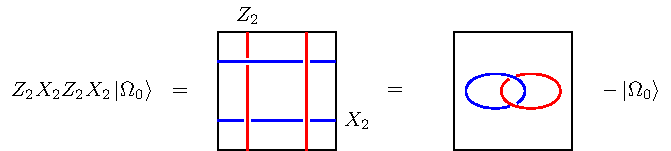
\includegraphics[scale=0.9]{anyons_ground_state.pdf}
    
    
\end{frame}

\begin{frame}
    \frametitle{Summary}

    \begin{itemize}
        \item Quantum codes encode $k$ qubits into $n$ qubits. 
        \item Quantum codes allow for error correction 
        \item The Kitaev toric code encode $2g$ qubits into a spin lattice.  
        \item The Kitaev code has $e^{-\alpha N}$ probability of missing errors. 
        \item By moving anyons around, one can perform quantum operations on the qubits. 
        \item The anyon content of a theory is enough to define its topological order.
    \end{itemize}

\end{frame}


\bibliographystyle{plainnat}
\bibliography{reference}
\end{document} 
 
